\documentclass[a4paper,11pt, tikz]{article}
\usepackage[T1]{fontenc}
\usepackage[utf8]{inputenc}
\usepackage{lmodern}
\usepackage{xcolor}
\usepackage{textcomp}
%\usepackage{newspaper}
%\date{\today}
%\currentvolume{1430}
%\currentissue{6}
%\usepackage{times}
\usepackage{graphicx}
\usepackage{multicol}
\usepackage{etoolbox}
\usepackage{picinpar}
%uasage of picinpar:
%\begin{window}[1,l,\includegraphics{},caption]xxxxx\end{window}
%\usepackage{times}
%\usepackage[T1]{fontenc}
\usepackage[utf8]{inputenc}
%\usepackage[nohead, nomarginpar, margin=1in, foot=.25in]{geometry}
\usepackage{lmodern}
%\usepackage{fontspec}
\usepackage{setspace}
%\usepackage{fancyhdr}
\usepackage{everyshi}
\usepackage{pdfpages}
\usepackage{indentfirst}
\usepackage[hyphens]{url}
\usepackage{hyperref}
\usepackage{pdfpages}
\usepackage{pgfpages}
\usepackage{amssymb}
\usepackage{mathtools}
\usepackage{amsmath}
\usepackage[notextcomp]{stix}
 \usepackage{paracol}
 \usepackage{stmaryrd}
 \usepackage{xurl}
 \usepackage{wasysym}
\usepackage{tikz}
 \usetikzlibrary{cd}
\usepackage[left=2cm, right=2cm, top=2cm, bottom=2cm]{geometry}
%\pagestyle{fancy}
%\lhead{Curriculum vitae, Anamitro Biswas}
%\chead{}
%\rhead{}
%\lfoot{}
%\cfoot{\thepage}
%\rfoot{}
%\makeatletter
%\renewcommand{\@chapapp}{Document}
%\makeatother
%\renewcommand\refname{\enhead\color{red}{References:}}
%\renewcommand{\headrulewidth}{0.4pt}
%\renewcommand{\footrulewidth}{0.4pt}
%\newfontfamily\bn{TiroBangla-Regular.ttf}[Script=Bengali]
%\newfontfamily\enhead{RubikDoodleShadow-Regular.ttf}[Script=Latin]
%\setmainfont{cmunrm.ttf}[Script=Latin]
%\newfontfamily\bn{TiroBangla-Regular.ttf}[Script=Bengali]
%\newfontfamily\latinfont{OfenbacherSchwabCAT.ttf}[Script=Latin]

\newcommand{\rel}{\text{ rel}}
\renewcommand{\S}{\mathbb{S}^}
\newcommand{\CP}{\mathbb{C}\text{P}^}
\newcommand{\RP}{\mathbb{R}\text{P}^}
\newcommand{\Gr}{\text{Gr}_}
\newcommand{\Cech}{\operatorname{\check{C}ech}}
\newcommand{\VR}{\operatorname{\mathcal{V}\mathcal{R}}}

%BRACKETS:
\newcommand{\lb}{\left(}
\newcommand{\rb}{\right)}
\newcommand{\lc}{\left\lbrace}
\newcommand{\rc}{\right\rbrace}
\newcommand{\ls}{\left[}
\newcommand{\rs}{\right]}
\renewcommand{\la}{\left\langle}
\renewcommand{\ra}{\right\rangle}


%CATEGORY THEORY:
\newcommand{\Ab}{\mathcal{A}\mathfrak{b}}
\newcommand{\Top}{\mathcal{T}\mathfrak{o}\mathfrak{p}}

%CHARACTERISTIC CLASSES
\newcommand{\diff}{\operatorname{D}}
\newcommand{\Man}{\M\mathfrak{a}\mathfrak{n}}
\newcommand{\smMan}{\M\mathfrak{a}\mathfrak{n}^\infty}
\newcommand{\sm}{\mathcal{C}^\infty}

%DASH AND BAR:
\newcommand{\dash}{^\prime}
\newcommand{\ddash}{^{\prime\prime}}
\newcommand{\tdash}{^{\prime\prime\prime}}

%FIELDS:
\newcommand{\reals}{\mathbb{R}}
\newcommand{\bC}{\mathbb{C}}
\newcommand{\complex}{\mathbb{C}}
\newcommand{\bG}{\mathbb{G}}
\newcommand{\bP}{\mathbb{P}}
\newcommand{\bE}{\mathbb{E}}
\newcommand{\bH}{\mathbb{H}}
\newcommand{\bF}{\mathbb{F}}
\newcommand{\bN}{\mathbb{N}}
\newcommand{\naturals}{\mathbb{N}}
\newcommand{\Z}{\mathbb{Z}}
\newcommand{\integers}{\mathbb{Z}}

%FUZZY TOPOLOGY:
\newcommand{\nphi}{\bigodot}

%GREEK UPPERCASE:
\newcommand{\Lm}{\Lambda}
\newcommand{\G}{\Gamma}
\newcommand{\D}{\Delta}
\newcommand{\Th}{\Theta}
\newcommand{\F}{\Phi}
\newcommand{\W}{\Omega}

%GREEK LOWERCASE:
\newcommand{\m}{\mu}
\newcommand{\lm}{\lambda}
\renewcommand{\l}{\lambda}
\newcommand{\vs}{\varsigma}
\newcommand{\g}{\gamma}
\renewcommand{\t}{\tau}
\renewcommand{\a}{\alpha}
\renewcommand{\b}{\beta}
\newcommand{\e}{\varepsilon}
\newcommand{\dt}{\delta}
\newcommand{\f}{\varphi}
\newcommand{\z}{\zeta}
\newcommand{\s}{\sigma}
\newcommand{\p}{\pi}
\newcommand{\y}{\eta}
\renewcommand{\th}{\theta}
\newcommand{\dl}{\partial}
\newcommand{\w}{\omega}

%GROUP THEORY:
\newcommand{\inv}{^{-1}}
\newcommand{\GL}{\operatorname{GL}}
\newcommand{\SL}{\operatorname{SL}}

%HOMOLOGICAL ALGEBRA:
\newcommand{\Hom}{\operatorname{Hom}}
\newcommand{\Ext}{\operatorname{Ext}}
\newcommand{\im}{\operatorname{im}~}
%\newcommand{\lsft}{shift left=1.5ext}

%HOMTOPY GROUPS:
\newcommand{\htopo}{\mathcal{H}\mathfrak{o}\mathcal{T}\mathfrak{o}\mathfrak{p}_*}
\newcommand{\topo}{\mathcal{T}\mathfrak{o}\mathfrak{p}_*}
\newcommand{\htop}{\mathcal{H}\mathfrak{o}\mathcal{T}\mathfrak{o}\mathfrak{p}}
\newcommand{\cattop}{\mathcal{T}\mathfrak{o}\mathfrak{p}}


%LINEAR ALGEBRA
%\newcommand{\b}{\textbf{}}


%LOGIC:
\renewcommand{\implies}{\Rightarrow}

%MATHCAL:
\newcommand{\A}{\mathcal{A}}
\newcommand{\B}{\mathcal{B}}
\newcommand{\C}{\mathcal{C}}
\newcommand{\cD}{\mathcal{D}}
\newcommand{\E}{\mathcal{E}}
\newcommand{\cF}{\mathcal{F}}
\newcommand{\cG}{\mathcal{G}}
\newcommand{\Hy}{\mathcal{H}}
\newcommand{\I}{\mathcal{I}}
\newcommand{\J}{\mathcal{J}}
\newcommand{\List}{\mathcal{L}}
\newcommand{\M}{\mathcal{M}}
\newcommand{\N}{\mathcal{N}}
\newcommand{\R}{\mathcal{R}}
\newcommand{\Pa}{\mathcal{P}}
\newcommand{\La}{\mathcal{L}}
\newcommand{\Ta}{\mathcal{T}}
\newcommand{\mcS}{\mathcal{S}}
\newcommand{\V}{\mathcal{V}}
\newcommand{\X}{\mathcal{X}}
\newcommand{\Y}{\mathcal{Y}}

%MATHFRAK:
\newcommand{\Mf}{\mathfrak{M}}
\newcommand{\Nf}{\mathfrak{N}}
\newcommand{\gf}{\mathfrak{g}}
\newcommand{\mfi}{\mathfrak{i}}
\newcommand{\mfj}{\mathfrak{j}}
\newcommand{\mfa}{\mathfrak{A}}

%MATH BOLD:
\newcommand{\bfa}{\mathbf{a}}
\newcommand{\bfb}{\mathbf{b}}
\newcommand{\bfg}{\mathbf{g}}
\newcommand{\bft}{\mathbf{t}}
\newcommand{\bfx}{\mathbf{x}}
\newcommand{\bfy}{\mathbf{y}}
\newcommand{\bfzero}{\mathbf{0}}


%MAPS:
\newcommand{\tends}{\rightarrow}
\newcommand{\id}{\operatorname{id}}
\newcommand{\incl}{\hookrightarrow}



%SET THEORY:
\newcommand{\cl}{\overline}
\newcommand{\intr}{^\circ}
\newcommand{\ir}{^\text{int}}
\newcommand{\comp}{^C}
\newcommand{\where}{\bigg| }
\newcommand{\lmid}{\left\vert}
\newcommand{\rmid}{\right\vert}

%HEADINGS:
\newtheorem{thm}{Theorem}
\newtheorem{prop}[thm]{Proposition}
\newtheorem{cor}[thm]{Corollary}
\newtheorem{defn}[thm]{Definition}
\newtheorem{obs}[thm]{Observation}
%\newtheorem{prop}[thm]{Proposition}
\newtheorem{lem}[thm]{Lemma}
\newtheorem{conj}[thm]{Conjecture}
\newtheorem{claim}[thm]{Claim}
\newtheorem{note}[thm]{Note}
\newtheorem{notation}[thm]{Notation}
\newtheorem{rem}[thm]{Remark}
\newtheorem{prob}[thm]{Problem}
\newcommand{\Ob}{\text{Ob}}
\newcommand{\Eq}{\text{Eq}}

%\setmainfont{Cormorant Garamond SemiBold}
\urlstyle{same}
\usepackage{tikzpagenodes}
\usepackage{tikz}
\usepackage{eso-pic}
\begin{document}
\title{Bundles}
\author{Anamitro Biswas\\Webpage: \url{https://anamitro.github.io}}
\maketitle
\section{Fibrations}
%\begin{defn}
\noindent{}If $\lb B, b_0\rb$ is a connected based space, a surjective continuous map $p:E\tends B$ is called a \emph{locally trivial fibration} with \emph{fiber} $F$ if
\begin{enumerate}
\item $p^{-1}\lb b_0\rb=F$;
\item every $x\in B$ has an open neighbourhood $U_x\subset B$ and a fiber-preserving homeomorphism $\psi_{U_x}:p^{-1}\lb U_x\rb\tends U_x\times F$ such that the following diagram commutes:
\begin{equation*}
\begin{tikzcd}
E\supset &p^{-1}\lb U_x\rb \ar[d, "p"] \ar[r, "\psi_{U_x}", "\cong"'] & U_x\times F\ar[dl, "\p_1"] & \subset B\times F \\
x\in & U_x & \subset B &
\end{tikzcd}
\end{equation*}
\end{enumerate}
%\end{defn}
The idea of a fiber bundle is something like a quotient map, loosening the condition from an equivalence relation to just a fibration map, and requiring the commutativity with that map:
  \begin{center}
    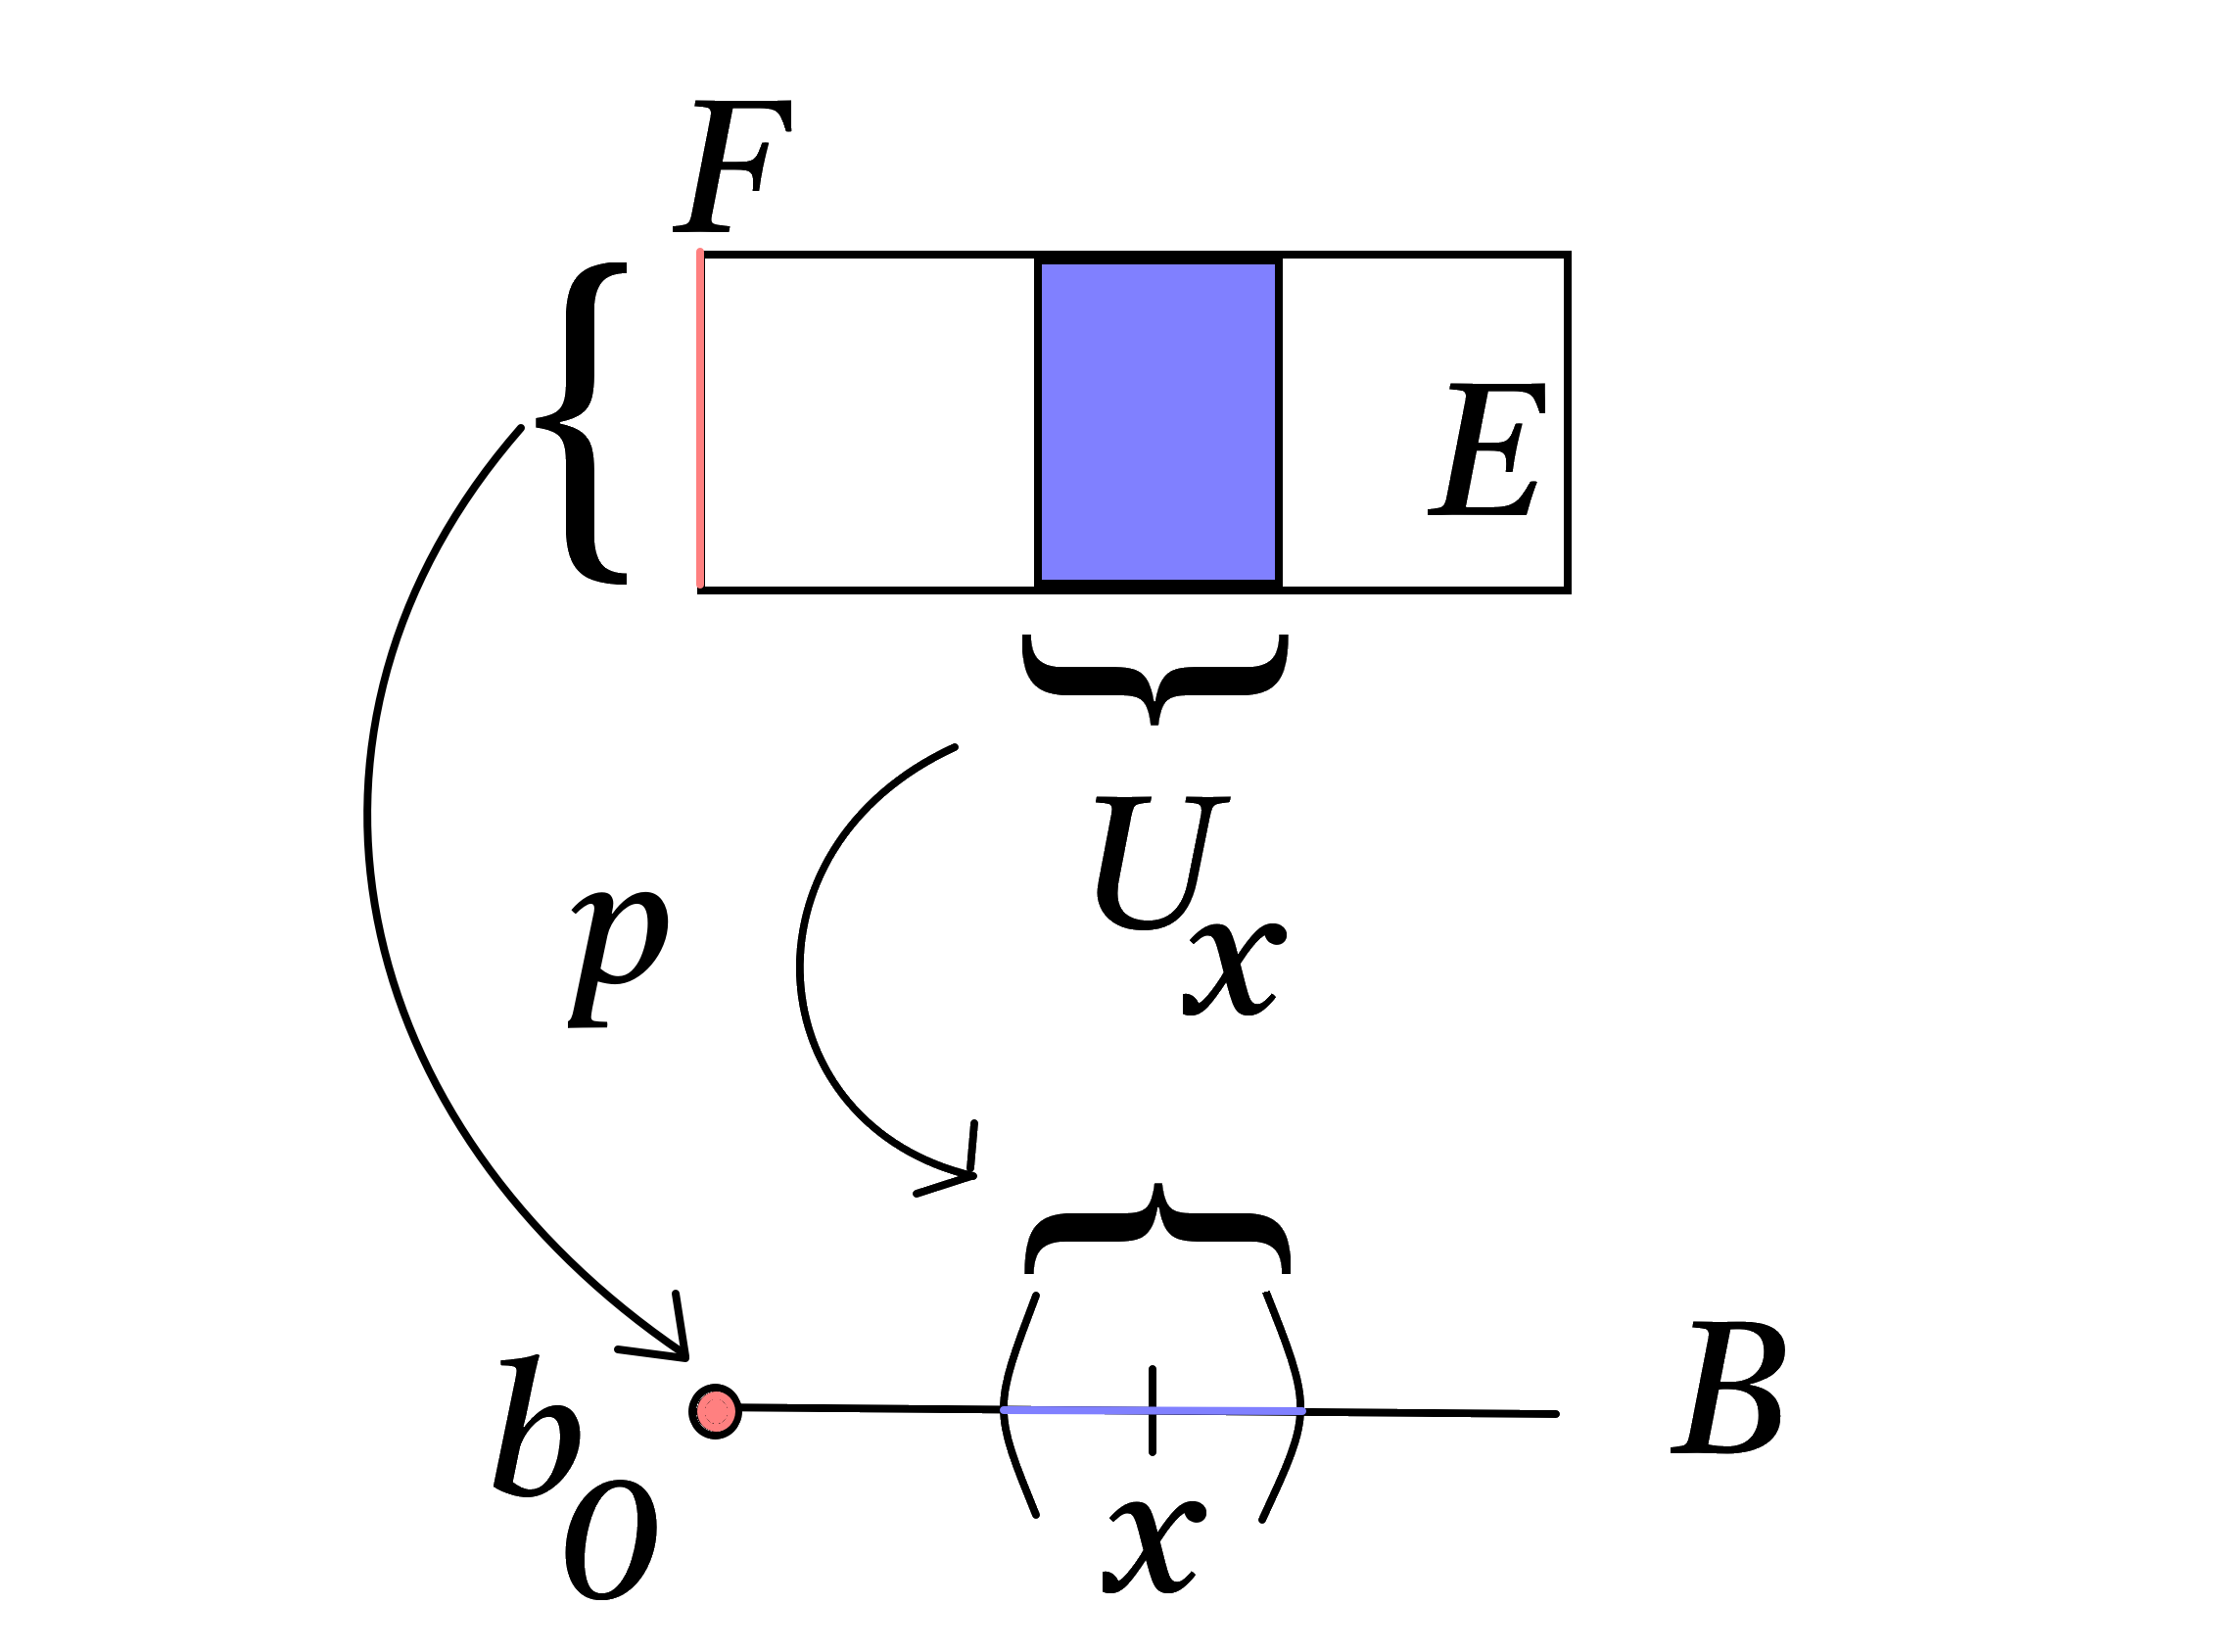
\includegraphics[width=0.25\textwidth]{fiber_bundle.png}
  %  \caption{}
  \end{center}
  The space $B$ is called the \emph{base space} and $E$ is called the \emph{total space}. This data for a \emph{fiber bundle} is denoted by the triple $\lb F, E, B\rb$.

A \emph{map} or \emph{morphism} of fiber bundles, $\F=\lb \cl{\f}, \f\rb:\lb F_1, E_1, B_1\rb\tends \lb F_2, E_2, B_2\rb$ preserves base points and is such that the following diagram commutes
\begin{equation*}
\begin{tikzcd}
E_1\ar[d, "p_1"]\ar[r, "\cl{\f}"] & E_2\ar[d, "p_2"]\\
B_1 \ar[r, "\f"] & B_2
\end{tikzcd}
\end{equation*}
Such a map of fibrations determines a continuous map $\f_0:F_1\tends F_2$. It is an \emph{isomorphism} if, additionally, we have $\F^{-1}:\lb F_2, E_2, B_2\rb\tends \lb F_1, E_1, B_1\rb$ such that $\F\circ \F\inv=\F\inv\circ \F=1$.
\begin{itemize}
  \item[\textleaf]The projection map $\pi:X\times F\tends X$ is the \emph{trivial fibration} over $X$ with fiber $F$.
  \item[]Any fibration that is isomorphic to the trivial fibration is trivial as well.
  \item[\textleaf]Let $(1,0)$ be the base-point of $\S 1 \subset \complex$ and consider the map $f_n:\S 1\tends \S 1; z\mapsto z^n$. The fiber of $f_n$ are the $n$th roots of unity.
  \item[]However, this bundle is not trivial. Consider the possible map to the trivial bundle
  \begin{equation*}
\begin{tikzcd}
\S 1\times F\ar [r, "\cl{\y}"] \ar[d, "\p_1"] & \S1\ar[d, "f_n"]\\
\S 1\ar[r, "\y"] & \S1
\end{tikzcd}
\end{equation*}
where $|F|=n$, so $\S1\times F$ is disconnected while $\S1$ is not; so there can be no isomorphism $\cl{\y}$ between them.
\item[\textleaf]The map $\exp:\reals\tends \S1;t\mapsto e^{2\p i t}$ is a locally trivial fibration, whose fiber is $\integers$. It makes the real line kind of a spiral over $\S1$. It is a covering map, and hence a locally trivial fibration. This fibration is also not trivial.
\item[\textleaf]A \emph{covering space} is a locally trivial fibration with discrete fiber.
\item[\textleaf]We can define $\RP n=\S n/\sim $, that identifies the antipoles. The projection map $p:\S n\tends \RP n$ is a locally trivial fibration with fiber the two-point set. This is also non-trivial. The complex analogue will also work: $\CP n=\S{2n+1}/\sim$ where $x\sim ux$ for $u\in \S1\subset \complex$; the locally trivial fibration $p:\S{2n+1}\tends \CP n$ has fiber $\S1$.
\item[\textleaf]In the M\"{o}bius band $M=[0,1]\times [0,1]/\sim$ where $(t,0)\sim(1-t, 1)\forall t\in I$, let $C=\lc \lb \frac{1}{2}, s\rb\in M\rc$ be the centre circle. The projection $p:M\tends C; \lb t,s\rb\mapsto\lb \frac{1}{2}, s\rb$ is a locally trivial fibration with fiber $[0,1]$.
  \end{itemize}
  
    \section{Smooth manifolds}
\noindent{}Let $\reals^n$ be the affine $n$-space, and any function defined one an open set $U\subset \reals^n$ with values in $\reals^k$ is \emph{smooth} if its partial derivatives of all orders exist and are continuous,i.e., it is differentiable of class $C^\infty$. In case we need to talk about an infinite-dimensional coordinate space, $\reals^A$ can be thought of as the vector space consisting of all functions ${\bf{x}} :A\tends \reals$. $\reals^n$ is a special case where $A=\lc 1, 2,\dots, n\rc$. The $\a$th coordinate of $\bf{x}$ is the value of vector $x\in\reals^A$ on $\a\in A$. For a function $f:Y\tends \reals^A$, the $\a$th coordinate of $f(y)$ will be denoted by $f_\a(y)$. Now it is but routine to topologize $\reals^A$ as a Cartesian product of $|A|$ copies of $\reals$. For any subset $M\subset \reals^A$, it has the relative topology. Thus a function $f:Y\tends \reals^A$ is continuous iff each associate function $f_\a:Y\tends \reals$ is continuous. For $U\subset\reals^n$, a function $f:U\tends M\subset\reals^A$ is \emph{smooth} if each of the associated functions $f_\a:U\tends\reals$ is smooth. If $f$ is smooth then $\dfrac{\dl f}{\dl u_i}$ can be defined as a smooth function $U\tends\reals^A$ whose $\a$th coordinate is $\dfrac{\dl f_\a}{\dl u_i}$ for $i\in\lc 1,2,\dots, n\rc$.

A subset $M\subset\reals^A$ is a smooth manifold of dimension $n\geq 0$ if for each $x\in M$ there exists a smooth function $h:U\tends \reals^A$ defined on an open set $U\subset\reals^n$ such that
\begin{itemize}
  \item[(i)]$h:U\xrightarrow{\text{homeomorphism}} V^\text{open}\subset M$ where $x\in V$;
  \item[(ii)]for each $u\in U$ the matrix $\ls\dfrac{\dl h_\a(u)}{\dl u_j}\rs$ has rank $n$. In other words, the vectors $\lc\dfrac{\dl h}{\dl u_j}\rc_{j\in[n]}$, evaluated at $u$, must be linearly independent. [Does this basically mean that no dimension is lost in the mapping?]
\end{itemize}
The image $h(u)=V$ of such a mapping is called a \emph{coordinate neighbourhood} of $M$, and the triple $\lb U, V, h\rb$ is called a \emph{local parametrization} of $M$. The inverse $h\inv:V\tends U\subset\reals^n$ is called a \emph{chart} which is a \emph{local coordinate system} of $M$. The most classical and familiar examples of smooth manifolds are curves and surfaces in $\reals^3$.

If $\lb U, V, h\rb$ and $\lb U', V', h'\rb$ are two local parametrizations of $M$ such that $V\cap V'\neq\phi$. Then $\f:\lb\reals^n\supset\rb\lb h'\rb^{-1}\lb V \cap V'\rb\tends h\inv\lb V \cap V'\rb\subset \reals^n; u'\mapsto h\inv\lb h'\lb u\rb\rb$ is a smooth mapping. To see this, consider arbitrary $\cl{x}=h\lb \cl{u}\rb=h'\lb \cl{u'}\rb\in V \cap V'$. Choose indices $\a_1,\dots, \a_n$ such that $\ls \dfrac{\dl h_{\a_i}}{\dl u_j}\rs_{n\times n}$ evaluated at $\cl{u}$ is non-singular (how am I sure that such $n$ indices exist? Is this because no dimension is lost in the mapping for a manifold?). It follows from inverse function theorem that one can solve for $u_1, \dots, u_n$ as smooth functions $u_j=f_j\lb h_{\a_1}\lb u\rb, \dots, h_{\a_n}\lb u\rb\rb$ for $u$ in some neighbourhood of $\cl{u}$. This gives us $u=f\lb h_{\a_1}\lb u\rb, \dots, h_{\a_n}\lb u\rb\rb$, and setting $h(u)=h'\lb u'\rb$, it follows that the function $u'\mapsto h\inv h'\lb u'\rb=f\lb h_{\a_1}'\lb u'\rb, \dots, h_{\a_n}'\lb u'\rb\rb$ is smooth throughout some neighbourhood of $u'$.

Consider two smooth manifolds $M\subset \reals^A$ and $N\subset \reals^B$, and let $\cl{x}\in M$ and $\lb U, V, h\rb$ be a local parametrization fo $M$ with $\cl{x}=h\lb \cl{u}\rb$. A function $f:M\tends N$ is said to be \emph{smooth} at $\cl{x}$ if the composition $f\circ h:U\tends N\subset \reals^B$ is smooth throughout some neighbourhood of $\cl{u}$. This definition does not depend on the choice of local parametrization. The function $f:M\tends N$ is \emph{smooth} if it is smooth at $x$ for every $x\in M$. It's a \emph{diffeomorphism} if it is additionally bijective and $f\inv$ is also smooth, i.e., a criterion of both-way smoothness imposed upon a homeomorphism. For a smooth manifold $M$, $\id_M$ is always smooth. Composition of two smooth maps $M\xrightarrow{g}M'\xrightarrow{f}M''$ is also smooth.

If $M$ is a manifold, a \emph{smooth path} through fixed $\cl{x}\in M$ is a smooth function $p:\lb -\e, \e\rb\tends M\subset \reals^A$ such that $p(0)=\cl{x}$ for some $\e>0$. The \emph{velocity vector} of such a path is defined to be $\dfrac{dp}{dt}\where_{t=0}=\lb\dfrac{dp_\a}{dt}\lb 0\rb:a \in A\rb\in\reals^A$. A vector $v\in\reals^A$ is tangent to $M$ at $x$ if $v$ can be expressed as a velocity vector of some smooth path through $x$ in $M$. The vector $v$ might be identified with the collection of paths $p$ which have the common velocity vector $v$; this allows an intrinsic definition of tangent vector independent of the embedding in $\reals^A$. The set of all such tangent vectors will be called the tangent space of $M$ at $x$, denoted by $\diff M_x$. To describe the tangent space in terms of local parametrization $\lb U, V, h\rb$ with $h\lb \cl{u}\rb=\cl{x}$, a vector $v\in\reals^A$ is tangent to $M$ at $\cl{x}$ if and only if $v$ can be expressed as a linear combination of $\lc \dfrac{\dl h}{\dl u_i}\lb \cl{u}\rb\rc_{i\in[1, n]}$. Thus, the set of all such tangent vectors, called the \emph{tangent space} of $M$ at $x$, denoted by $\diff M_x$, is an $n$-dimensional vector space over $\reals$. The \emph{tangent manifold} of $M$ is defined to be the subspace $\diff M\subset M\times\reals^A$ consisting of all pairs $\lb x,v\rb$ with $x\in M$ and $v\in \diff M_x$. As a subset of $\reals^A\times\reals^A$ it is a smooth manifold of dimension $2n$.

Any map $f:M\tends N$ which is smooth at $x$ determines a linear map $\diff f_x$ from the tangent space $\diff M_x$ to $\diff N_{f(x)}$. To see this, consider in $\diff M_x$, $v=\dfrac{dp}{dt}\where_{t=0}$, velocity vector of some smooth path $x\in M$, and define $\diff f_x(v)$ to be the velocity vector $\dfrac{d\lb f\circ p\rb}{dt}\where_{t=0}$ of the image path $f\circ p:\lb -\e, \e\rb\tends N$. This definition does not depend on the choice of $p$ [since we can think of the velocity vector as independent of embedding of $p$] and $\diff f_x$ is a linear mapping, called the \emph{derivative} or the \emph{Jacobian} of $f$ at $x$. In fact, in terms of local parametrization $\lb U, V, h\rb$ one has the explicit formula $\diff f_x\displaystyle\lb\sum_{i=1}^nc_i\dfrac{\dl h}{\dl u_i}\rb=\sum_{i=1}^n c_i\dfrac{\dl\lb f\circ h\rb}{\dl u_i}$ for $c_i\in\reals$.

Supposing $f:M\tends N$ to be smooth everywhere, combining all the Jacobians $\diff f_x$, one obtains a function $\diff f:\diff M\tends \diff N$ where $\diff f(x,v)=\lb f(x), \diff f_x(v)\rb$. If $\smMan$ be the category whose objects are smooth manifolds, and morphisms smooth maps, $D:\smMan\tends\smMan$ is a covariant functor. As a special consequence, if $f$ is a diffeomorphism from $M$ to $N$ the $\diff f$ is a diffeomorphism from $\diff M$ to $\diff N$.

Note that for the affine space $\reals^n$, $\diff\reals_x^n=\reals^n$, where in the latter case we can view $\reals^n$ as a vector space. [WHY?] In particular, for any $u\in \reals$, $\diff \reals_u=\reals$. For a smooth real-valued function $f:M\tends\reals$, its derivative is $\diff f_x:\diff M_x\tends\diff \reals_{f(x)}=\reals$ and so $\diff f_x\in\Hom_\reals\lb \diff M_x, \reals\rb$, the dual vector space. As an element of the dual space $\diff f_x=df(x)$ is called the \emph{total differential} of $f$ at $x$. From elementary calculus, we know Leibneitz rule to hold here: $\diff(fg)_x=f(x)\diff g_x+g(x)\diff f_x$. If $v\in \diff M_x$ (a tangent vector), $\diff f_x(v)\in\reals$ is called the \emph{directional derivative} of the real-valued function $f$ in the direction $v$. Let $\sm\lb M, \reals\rb$ be the vector space of all smooth real-valued functions on $M$. Keeping $\lb x, v\rb$ fixed we can vary $f$ over the vector space $\sm\lb M, \reals\rb$, and that gives a linear differential operator $X:\sm\lb M, \reals\rb\tends\reals;~f\mapsto\diff f_x\lb v\rb$. Leibnitz rule is automatically carried on: $X\lb fg\rb=f(x)X(g)+X(f)g(x)$.

One defect of the above presentation is that the ``smoothness'' of a manifold $M$ is made to depend on some particular embedding of $M$ in a coordinate space. However, we may canonically embed any smooth manifold $M$ in one preferred coordinate space, that does not involve and specific other embedding. Let $M\subset \reals^A$ and $F=\sm\lb M, \reals\rb$. Then we define $i:M\incl \reals^F;~{\mathbf{x}}\mapsto\lb f({\mathbf{x}})\ f\in F\rb$. [Seeing $\reals^F$ as set of all functions from $F$ to $\reals$, each element ${\mathbf{x}}$ of $M$ gives such a real-valued function on $M$; an element of $\reals^F$ whose $f$th coordinate is given by $f({\mathbf{x}})$.] Let $M_1=i\lb M\rb\subset \reals^F$. This $M_1$ is a smooth manifold in $\reals^F$ and the canonical map $i:M\tends M_1$ is a diffeomorphism. Any smooth manifold has a canonical embedding in an associated coordinate space. This suggests the following definition: Let $M$ be a set and $F$ be a collection of real-valued functions on $M$ which \emph{separates points}, i.e., for all $x\neq y\in M$ there exists $f\in F$ with $f(x)\neq f(y)$. Then $M$ can be identified with its image under the canonical imbedding $i:M\tends \reals^F$. Basically $M$ and $M_1$ are topologically same. The collection $F$ is a \emph{smoothness structure} on $M$ if the subset $i(M)\subset \reals^F$ is a smooth manifold [up to this, $F$ is a basis for a smoothness structure] and if $F=\sm\lb M, \reals\rb$.

\end{document}
%%%%%%%%%%%%%%%%%%%%%%%%%%%%%%%%%%%%%%%%%%%%%%%%%%%%%%%%%%%%%%%%%%%%%%%%%%%%%%%%%%%%%%%%%%%%%%%%%%%%%%%%%%%%%%%%%%%%%%%%%%%%%%%%%%%%%%%%%%%%%%%%%%%%%%%%%%%%%%%%%%%%%%%%%%%%%%%%%%%%%%%%%%%%%%%%%%%%%%%%%%%%%%%%%%
  \newpage
  \section{Exercise problems}
  \begin{itemize}
  \item[][Cohen]
  \item[1.]Verify that $\g_k$ is a $k$-dimensional real vector bundle over $\Gr k\lb\reals^n\rb$.
  \item[\textit{Soln.}]We have $\g_k=\lb F, E, \Gr{k}\lb\reals^n\rb\rb$ where $F$ is a $k$-dimensional subspace of $\reals^n$ and $E=\lc\lb W, \w\rb:W\in\right.$ $\left.\Gr{k}\lb\reals^n\rb, \w\in W\subset \reals^n\rc$. For $W\in\Gr k\lb\reals^n\rb$, $\g_k^{-1}\lb W\rb=\lc\lb W, \w\rb:\w\in W\rc\cong W$, a $k$-dimensional real vector space. Therefore, $\g_k$ is a $k$-dimensional real vector bundle over $\Gr{k}\lb\reals^n\rb$.
  \item[]
  \item[2.]Define the analogous bundle (which by abuse of notation we also call $\g_k$) over $\Gr{k}\lb\complex^n\rb$. Verify that this is a $k$-dimensional complex vector bundle over $\Gr{k}\lb\complex^n\rb$.
  \item[\textit{Soln.}]Consider the vector bundle $\g_k$ over $\Gr{k}\lb\complex^n\rb$ whose total space $E$ is the subspace of $\Gr{k}\lb\complex^n\rb\times\complex^n$ defined by $E=\lc\lb W, \w\rb:W\in\Gr{k}\lb\complex^n\rb, \w\in W\subset\complex^n\rc$. Then $\g_k$ is the vector bundle given by the natural projection $E\tends\Gr{k}\lb\complex^n\rb;\lb W, \w\rb\mapsto W$. For $W\in\Gr{k}\lb\complex^n\rb$, $\g_k^{-1}\lb W\rb=\lc \lb W, \w\rb:\w\in W\rc\cong W$, which is a $k$-dimensional complex vector space. Therefore, $\Gr{k}\lb\complex^n\rb$ is a $k$-dimensional complex vector bundle.
  \item[]
    \item[3.]Verify that $\RP{n-1}=\Gr1\lb\reals^n\rb$ and that the line bundle $\g_1$ defined above is a universal bundle. Do the analogous  exercise with $\CP{n-1}$ and $\Gr1\lb\complex^n\rb$.
    \item[\textit{Soln.}]In $\RP{n-1}$, we identify 1-dimensional subspaces of $\reals^n$, i.e., lines: the same we do for $\Gr1\lb \reals^n\rb$. Let $V_1\lb\reals^n\rb$ be the space of injective linear transformations from $\reals$ to $\reals^n$. These Stiefel manifolds can be thought of as spaces of $n\times 1$ matrices, i.e., $n$-dimensional vectors, of rank $1$; so basically, 1-dimensional lines. This space is given topology as a subspace of the appropriate vector space of matrices. We can define the equivalence relation in two ways: (i) Two transformations $A$ and $B$ are equivalent if they have the same image in $\reals^n$. Possible images are lines; so two transformations are equivalent when they end up in the same line (in essence, we ignore any scaling that might crop up). (ii) As matrices, $A\sim B$ if and only if $\exists~\l\in\GL(1, \reals)\cong \reals\setminus \lc 0\rc$ such that $A=\l B$. \textleaf~Then we define $\Gr{1}\lb\reals^n\rb=V_1\lb\reals^n\rb/\sim$. As for the vector bundle, let $E=\lc\lb W, \w\rb: W\in \Gr1\lb\reals^n\rb, \w\in W\text{, a line in }\reals^n\rc$ and $\g_1:E\tends \Gr{k}\lb\reals^n\rb; (W, \w)\mapsto W$ be the naturals projection. The fibre is an 1-dimensional line, so this is a real line bundle.
\paragraph{}We also have $\CP{n-1}=\complex^n/\sim$ where $x\sim ux$ for any $u\in\complex$ and for all $x\in \complex^n$. In $\Gr1\lb \complex^n\rb$ we identify the 1-dimensional $\complex$-vector spaces in $\complex^n$.

\item[][Milnor-Stasheff]
\item[1-A.]Let $M_1\subset \reals^A$ and $M_2\subset \reals^B$ be smooth manifolds. Show that $M_1\times M_2\subset \reals^A\times \reals^B$ is a smooth manifold and that the tangent manifold $\diff\lb M_1\times M_2\rb$ is canonically diffeomorphic to the product $\diff M_1\times \diff M_2$.
\item[]Note that a function $M\tends M_1\times M_2;~x\mapsto \lb f_1(x), f_2(x)\rb$ is smooth if and only if both $f_1$ and $f_2$ are smooth.
\item[]
\item[1-B.]
  \end{itemize}
  

%\end{document}
